% Editable native annotations around unchanged verified IDE photographs.
\par
\begin{figure}[htbp]
  \centering
  \newsavebox{\MARSrsapowerframeBox}
  \sbox{\MARSrsapowerframeBox}{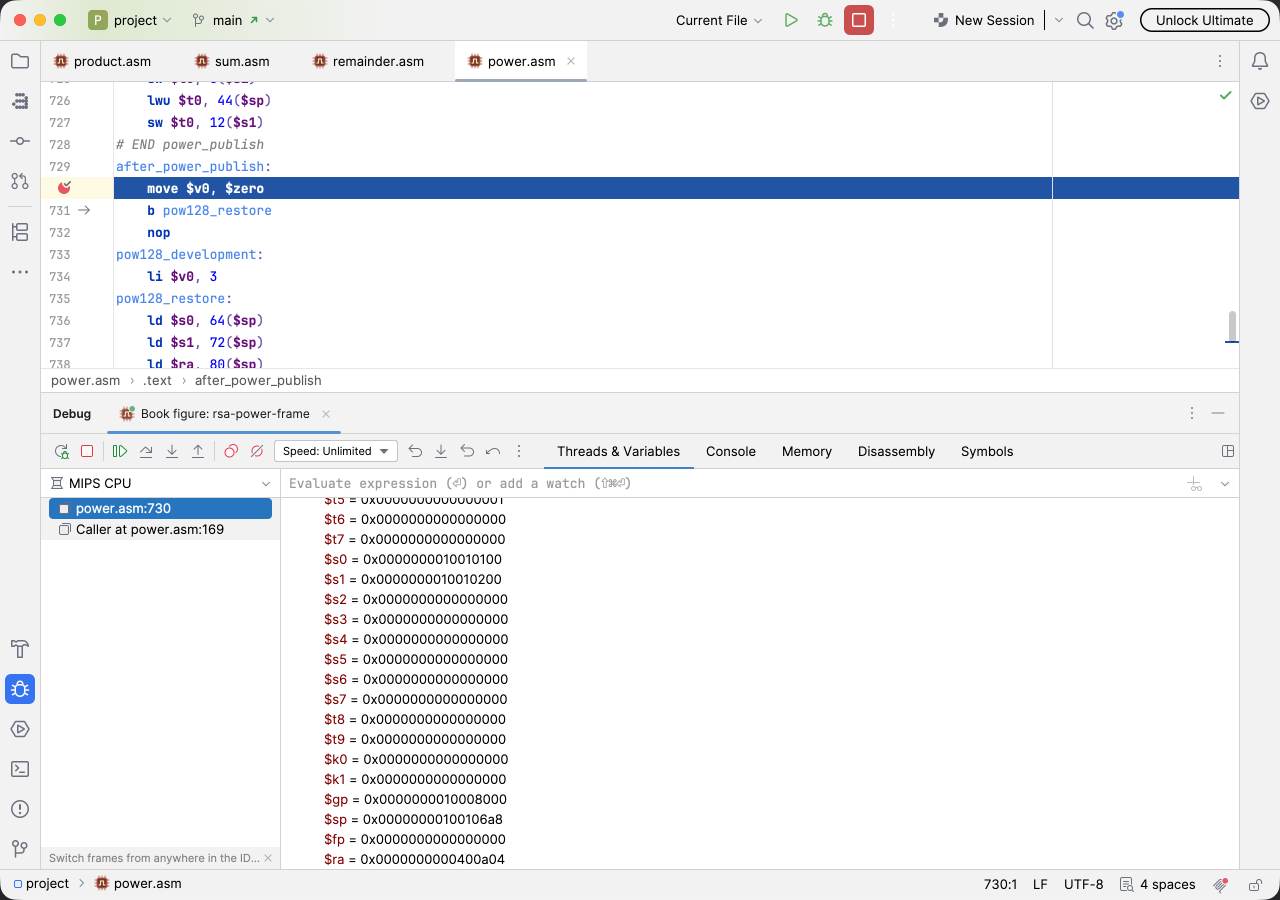
\includegraphics[artifact]{book/captures/027-rsa-arithmetic/f04/frame.png}}
  \newsavebox{\MARSrsapoweroutputBox}
  \sbox{\MARSrsapoweroutputBox}{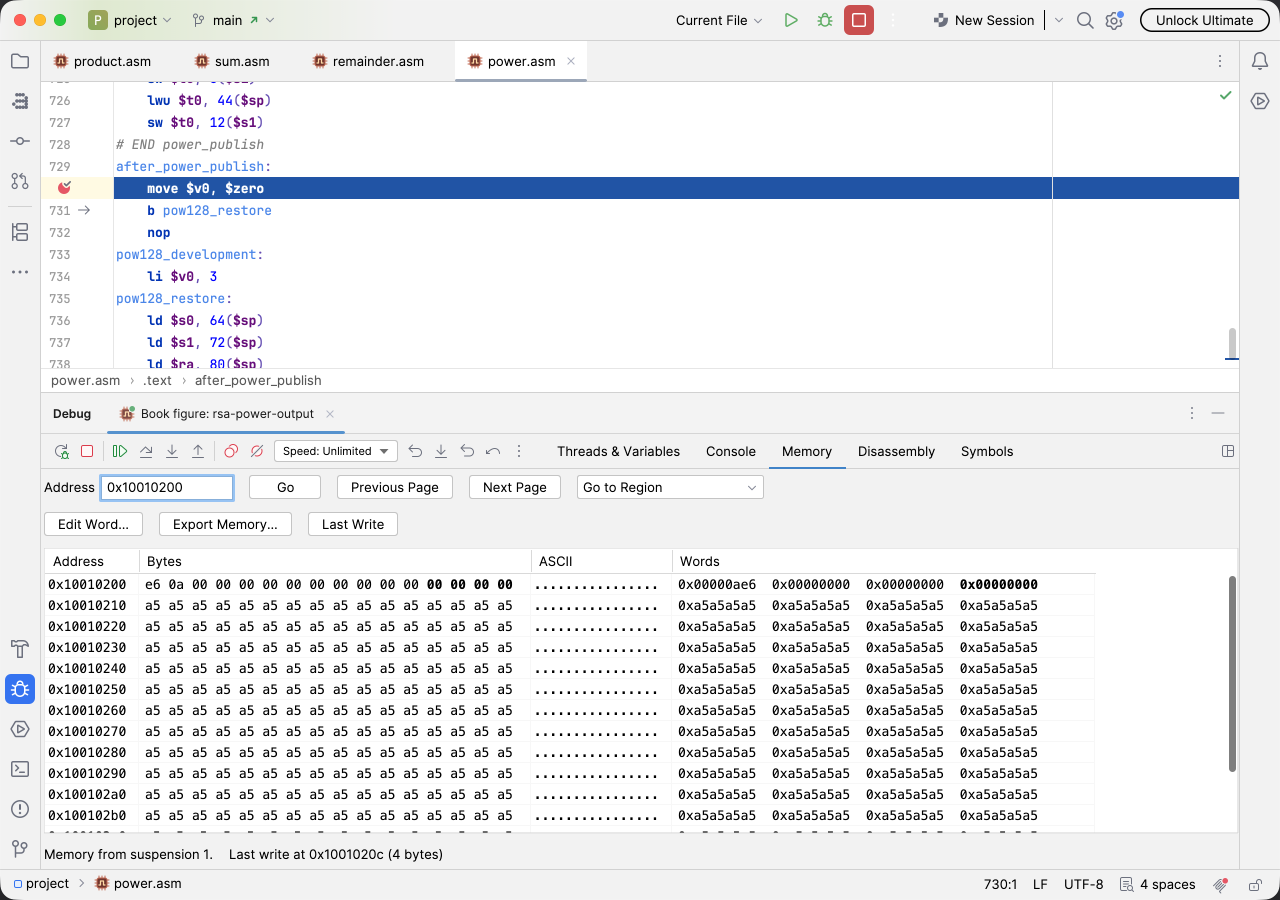
\includegraphics[artifact]{book/captures/027-rsa-arithmetic/f04/output.png}}
  \newsavebox{\MARSrsapowerprivateBox}
  \sbox{\MARSrsapowerprivateBox}{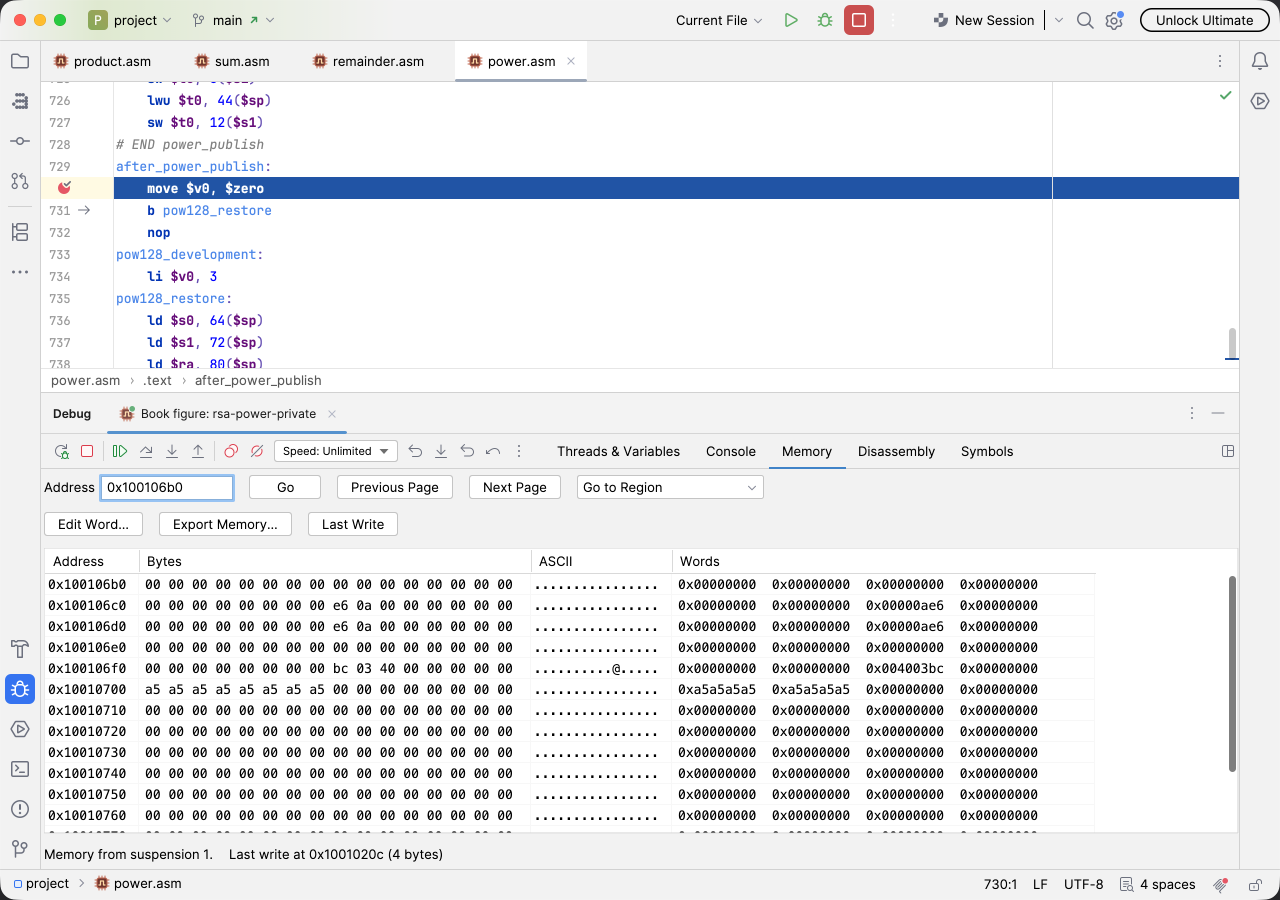
\includegraphics[artifact]{book/captures/027-rsa-arithmetic/f04/private.png}}
  \newsavebox{\MARSrsapowerinputsBox}
  \sbox{\MARSrsapowerinputsBox}{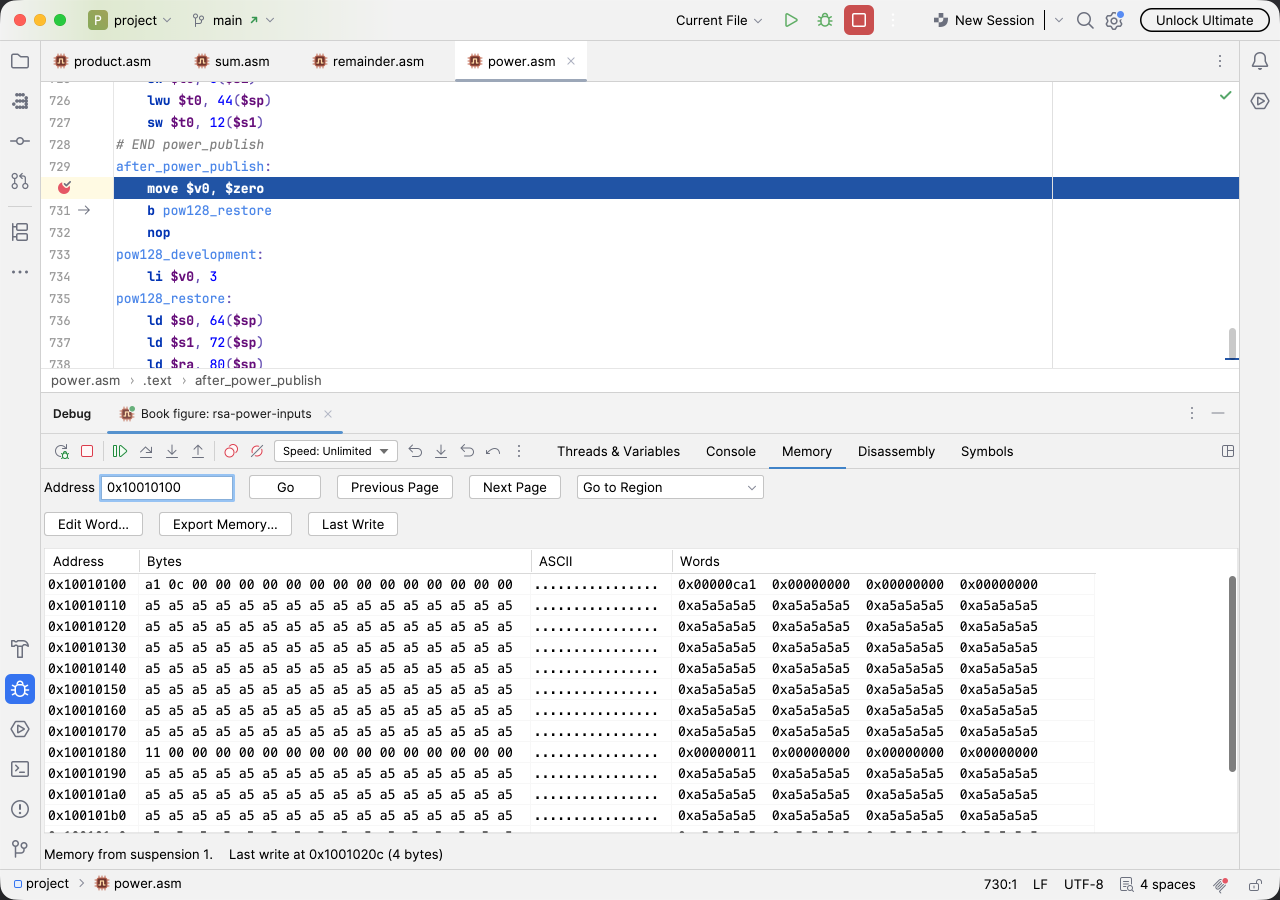
\includegraphics[artifact]{book/captures/027-rsa-arithmetic/f04/inputs.png}}
  \edef\MARSrsapowersourceLeft{\the\dimexpr0.036718750\wd\MARSrsapowerframeBox\relax}
  \edef\MARSrsapowersourceBottom{\the\dimexpr0.774444444\ht\MARSrsapowerframeBox\relax}
  \edef\MARSrsapowersourceRight{\the\dimexpr0.713281250\wd\MARSrsapowerframeBox\relax}
  \edef\MARSrsapowersourceTop{\the\dimexpr0.170000000\ht\MARSrsapowerframeBox\relax}
  \edef\MARSrsapowerframeLeft{\the\dimexpr0.246093750\wd\MARSrsapowerframeBox\relax}
  \edef\MARSrsapowerframeBottom{\the\dimexpr0.077777778\ht\MARSrsapowerframeBox\relax}
  \edef\MARSrsapowerframeRight{\the\dimexpr0.553906250\wd\MARSrsapowerframeBox\relax}
  \edef\MARSrsapowerframeTop{\the\dimexpr0.896666667\ht\MARSrsapowerframeBox\relax}
  \edef\MARSrsapoweroutputLeft{\the\dimexpr0.034375000\wd\MARSrsapoweroutputBox\relax}
  \edef\MARSrsapoweroutputBottom{\the\dimexpr0.334444444\ht\MARSrsapoweroutputBox\relax}
  \edef\MARSrsapoweroutputRight{\the\dimexpr0.584375000\wd\MARSrsapoweroutputBox\relax}
  \edef\MARSrsapoweroutputTop{\the\dimexpr0.608888889\ht\MARSrsapoweroutputBox\relax}
  \edef\MARSrsapowerprivateLeft{\the\dimexpr0.034375000\wd\MARSrsapowerprivateBox\relax}
  \edef\MARSrsapowerprivateBottom{\the\dimexpr0.311111111\ht\MARSrsapowerprivateBox\relax}
  \edef\MARSrsapowerprivateRight{\the\dimexpr0.584375000\wd\MARSrsapowerprivateBox\relax}
  \edef\MARSrsapowerprivateTop{\the\dimexpr0.608888889\ht\MARSrsapowerprivateBox\relax}
  \edef\MARSrsapowermodulusLeft{\the\dimexpr0.034375000\wd\MARSrsapowerinputsBox\relax}
  \edef\MARSrsapowermodulusBottom{\the\dimexpr0.334444444\ht\MARSrsapowerinputsBox\relax}
  \edef\MARSrsapowermodulusRight{\the\dimexpr0.584375000\wd\MARSrsapowerinputsBox\relax}
  \edef\MARSrsapowermodulusTop{\the\dimexpr0.608888889\ht\MARSrsapowerinputsBox\relax}
  \edef\MARSrsapowerexponentLeft{\the\dimexpr0.034375000\wd\MARSrsapowerinputsBox\relax}
  \edef\MARSrsapowerexponentBottom{\the\dimexpr0.147777778\ht\MARSrsapowerinputsBox\relax}
  \edef\MARSrsapowerexponentRight{\the\dimexpr0.584375000\wd\MARSrsapowerinputsBox\relax}
  \edef\MARSrsapowerexponentTop{\the\dimexpr0.795555556\ht\MARSrsapowerinputsBox\relax}
  \begin{tikzpicture}[alt={Six annotated details after_power_publish show all sixteen output bytes e6 0a followed by fourteen zero bytes, the still-active 96-byte frame, the exhausted private exponent and low power accumulator. The modulus is 3233 and original exponent 17. Restoration has not yet executed.}]
    \node[anchor=north west,inner sep=0,font=\small\bfseries] (source-title) at (6mm,0) {Next power instruction};
    \node[anchor=north west,inner sep=0] (source) at ([yshift=-1mm]source-title.south west) {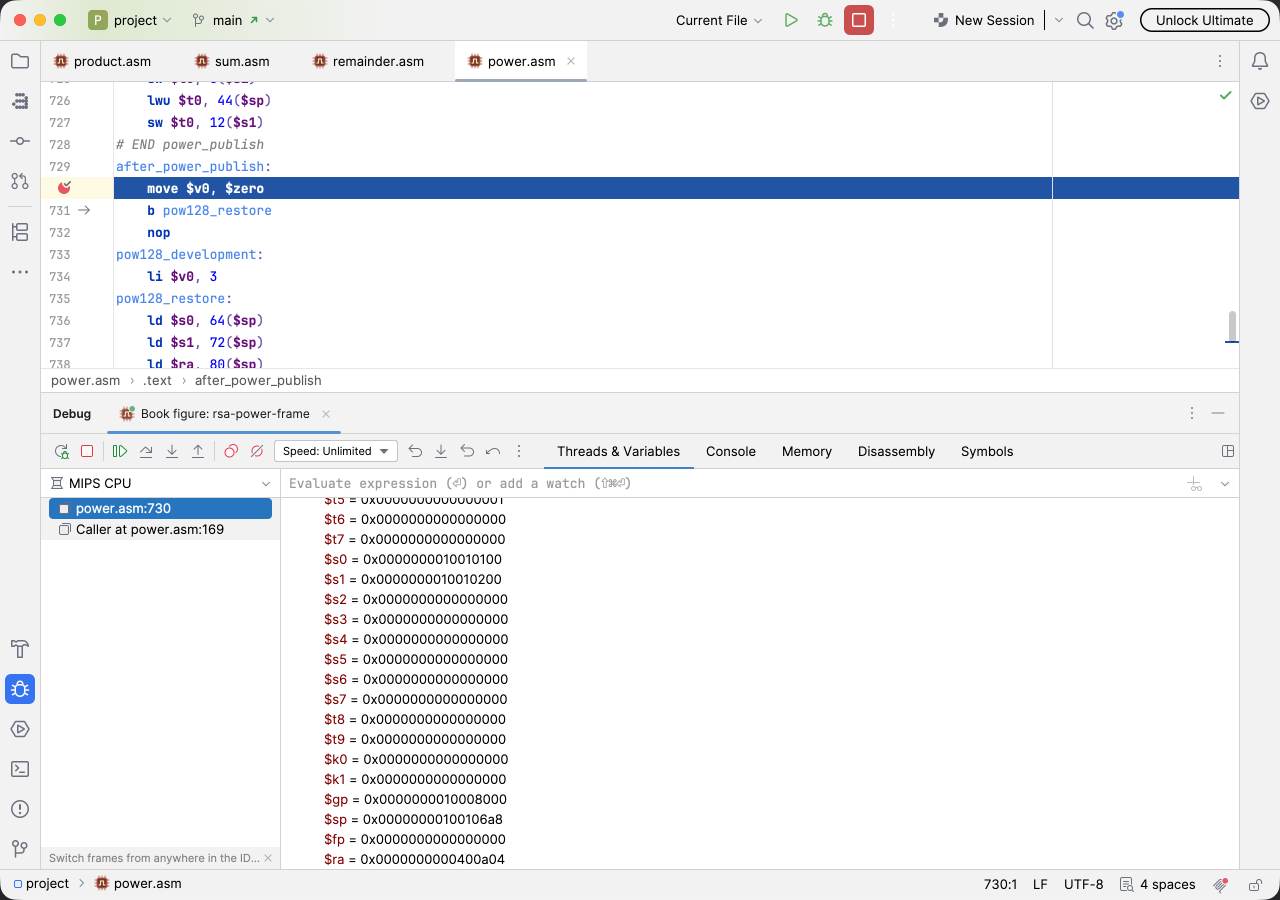
\includegraphics[width=0.54\linewidth,artifact,trim={\MARSrsapowersourceLeft{} \MARSrsapowersourceBottom{} \MARSrsapowersourceRight{} \MARSrsapowersourceTop{}},clip]{book/captures/027-rsa-arithmetic/f04/frame.png}};
    \begin{scope}[shift={(source.south west)},x={($(source.south east)-(source.south west)$)},y={($(source.north west)-(source.south west)$)}]
      \draw[black,line width=0.7pt] (0.215625000,0.080000000) rectangle (0.678125000,0.520000000);
      \node[draw=black,fill=white,circle,inner sep=1.5pt,font=\footnotesize] at ($(0.215625000,0.520000000)+(-3mm,0)$) {1};
    \end{scope}
    \node[anchor=north west,inner sep=0,font=\small\bfseries] (frame-title) at ([yshift=-1mm]source.south west) {Outer frame before restoration};
    \node[anchor=north west,inner sep=0] (frame) at ([yshift=-1mm]frame-title.south west) {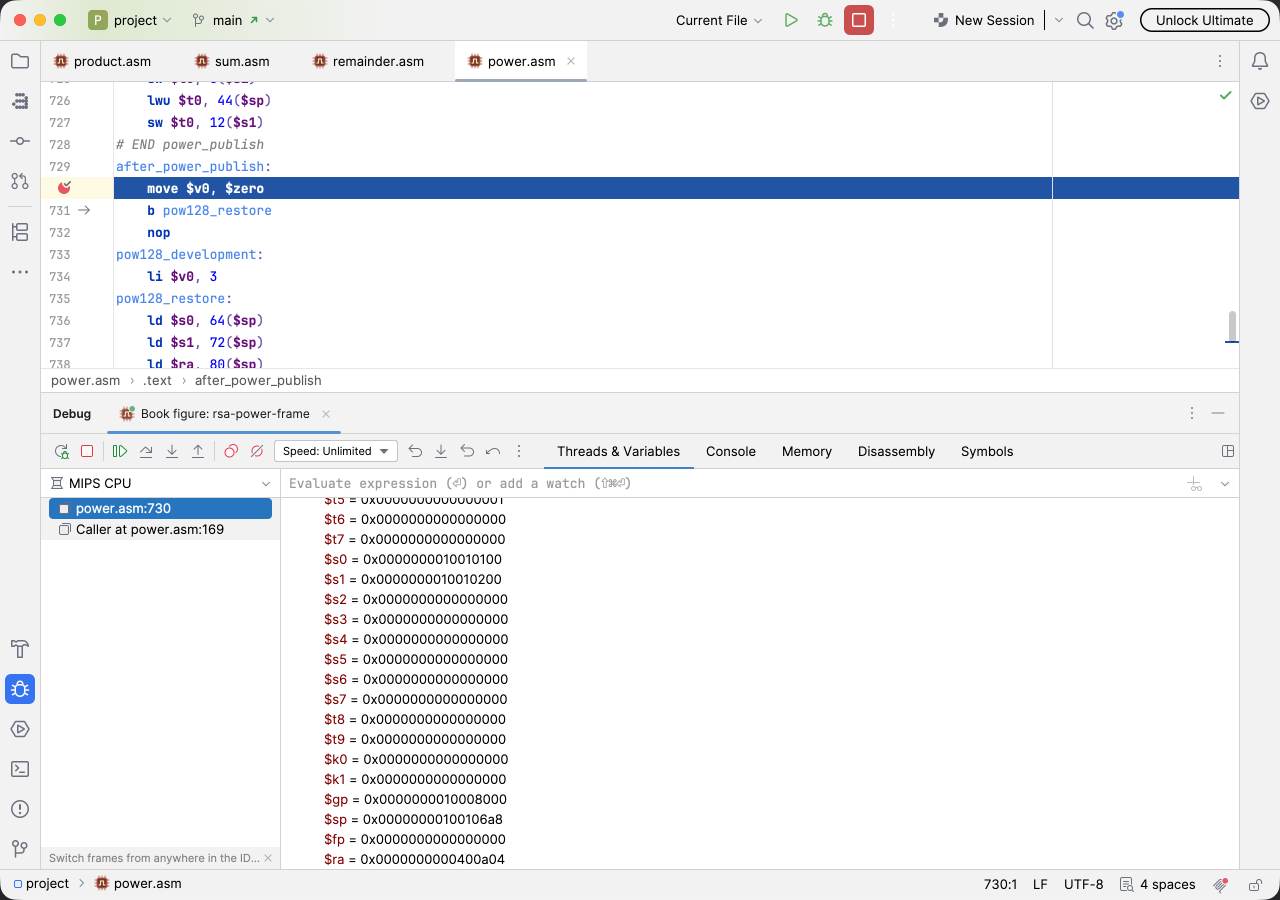
\includegraphics[width=0.44\linewidth,artifact,trim={\MARSrsapowerframeLeft{} \MARSrsapowerframeBottom{} \MARSrsapowerframeRight{} \MARSrsapowerframeTop{}},clip]{book/captures/027-rsa-arithmetic/f04/frame.png}};
    \begin{scope}[shift={(frame.south west)},x={($(frame.south east)-(frame.south west)$)},y={($(frame.north west)-(frame.south west)$)}]
      \draw[black,line width=0.7pt] (0.023437500,0.043478261) rectangle (0.738281250,0.913043478);
      \node[draw=black,fill=white,circle,inner sep=1.5pt,font=\footnotesize] at ($(0.023437500,0.913043478)+(-3mm,0)$) {2};
    \end{scope}
    \node[anchor=north west,inner sep=0,font=\small\bfseries] (output-title) at ([yshift=-1mm]frame.south west) {Complete published four-limb result};
    \node[anchor=north west,inner sep=0] (output) at ([yshift=-1mm]output-title.south west) {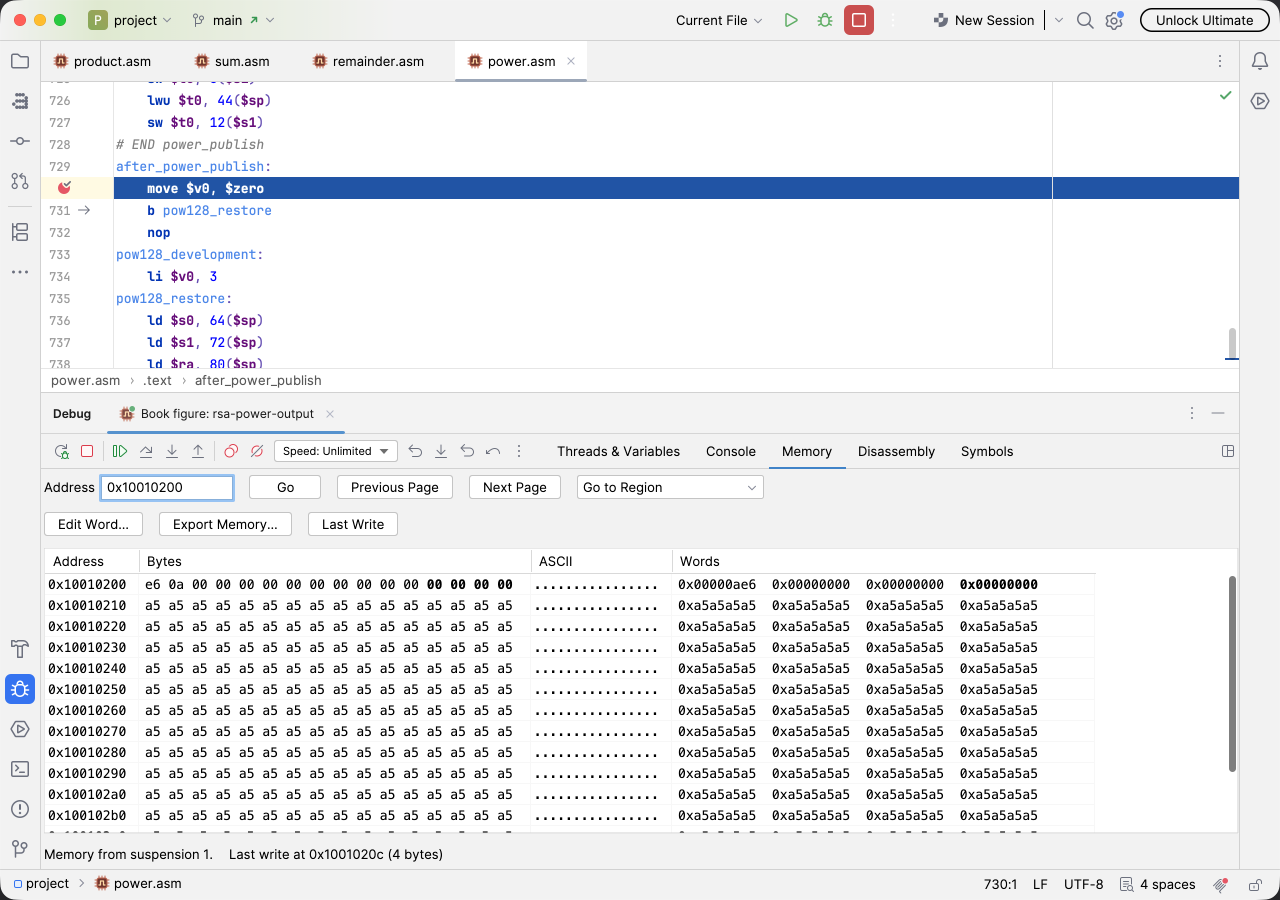
\includegraphics[width=0.84\linewidth,artifact,trim={\MARSrsapoweroutputLeft{} \MARSrsapoweroutputBottom{} \MARSrsapoweroutputRight{} \MARSrsapoweroutputTop{}},clip]{book/captures/027-rsa-arithmetic/f04/output.png}};
    \begin{scope}[shift={(output.south west)},x={($(output.south east)-(output.south west)$)},y={($(output.north west)-(output.south west)$)}]
      \draw[black,line width=0.7pt] (0.194672131,0.078431373) rectangle (0.997950820,0.490196078);
      \node[draw=black,fill=white,circle,inner sep=1.5pt,font=\footnotesize] at ($(0,0.490196078)+(-3mm,0)$) {3};
    \end{scope}
    \node[anchor=north west,inner sep=0,font=\small\bfseries] (private-title) at ([yshift=-1mm]output.south west) {Exhausted private exponent and accumulator};
    \node[anchor=north west,inner sep=0] (private) at ([yshift=-1mm]private-title.south west) {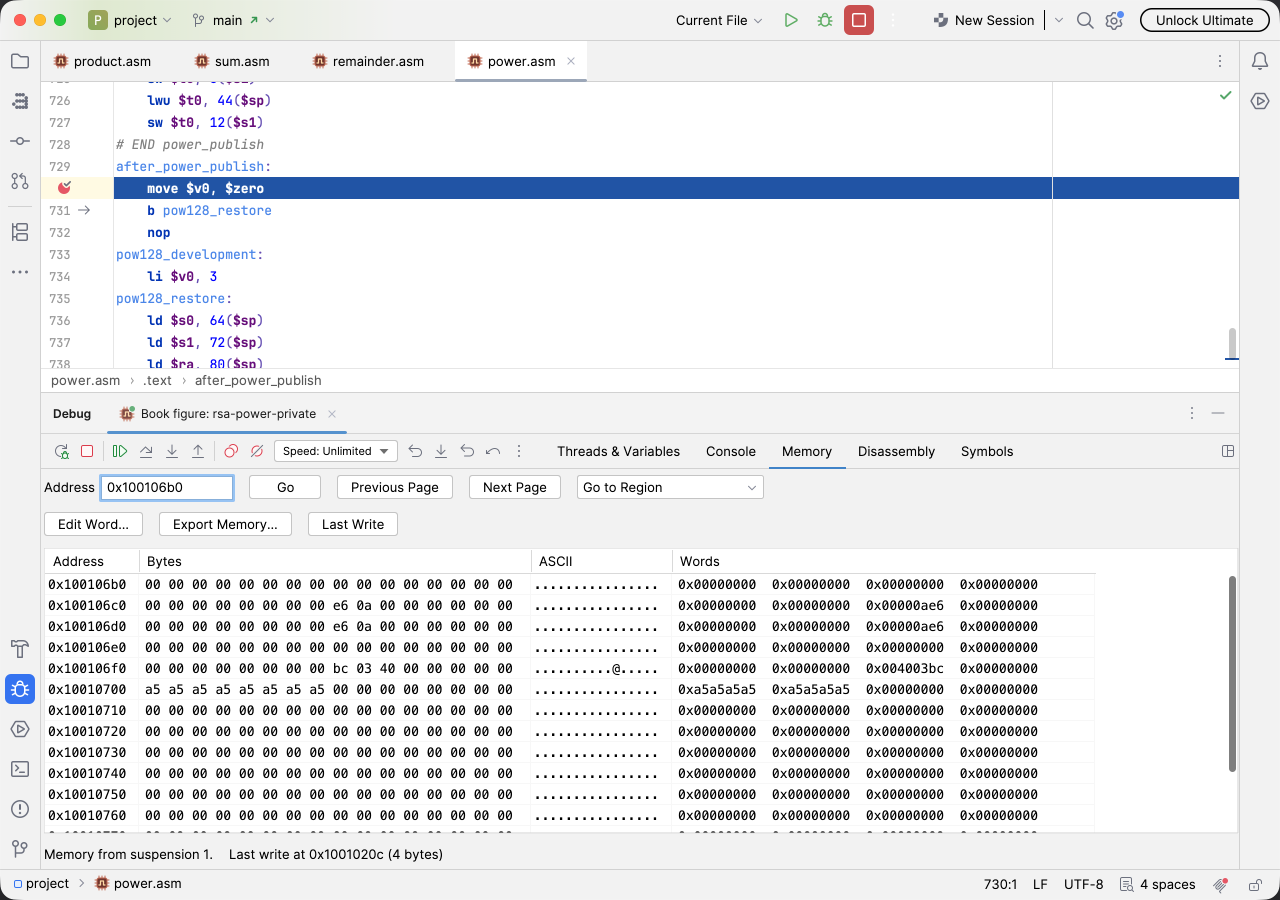
\includegraphics[width=0.84\linewidth,artifact,trim={\MARSrsapowerprivateLeft{} \MARSrsapowerprivateBottom{} \MARSrsapowerprivateRight{} \MARSrsapowerprivateTop{}},clip]{book/captures/027-rsa-arithmetic/f04/private.png}};
    \begin{scope}[shift={(private.south west)},x={($(private.south east)-(private.south west)$)},y={($(private.north west)-(private.south west)$)}]
      \draw[black,line width=0.7pt] (0.194672131,0.055555556) rectangle (0.997950820,0.638888889);
      \node[draw=black,fill=white,circle,inner sep=1.5pt,font=\footnotesize] at ($(0,0.638888889)+(-3mm,0)$) {4};
    \end{scope}
    \node[anchor=north west,inner sep=0,font=\small\bfseries] (modulus-title) at ([yshift=-1mm]private.south west) {Original modulus};
    \node[anchor=north west,inner sep=0] (modulus) at ([yshift=-1mm]modulus-title.south west) {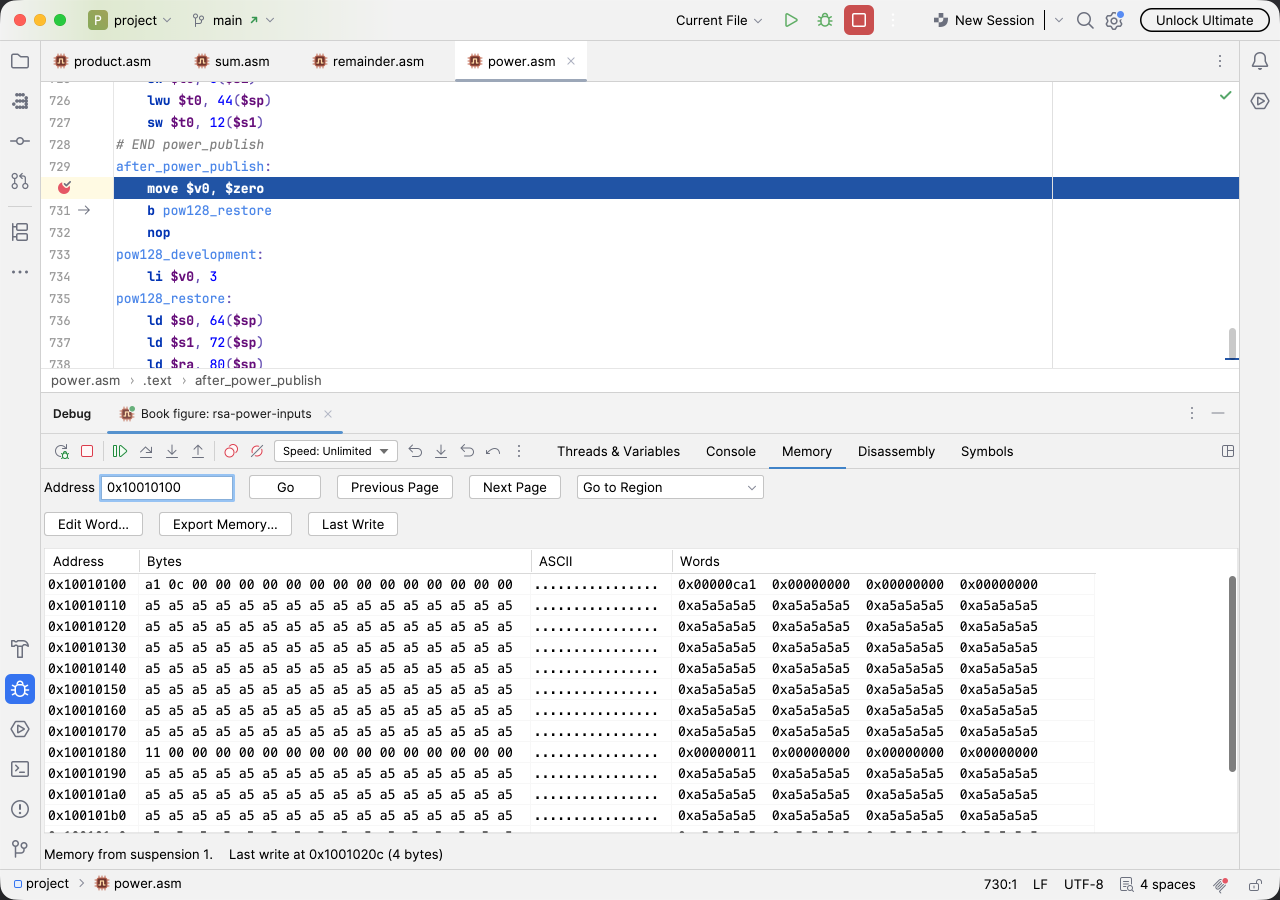
\includegraphics[width=0.84\linewidth,artifact,trim={\MARSrsapowermodulusLeft{} \MARSrsapowermodulusBottom{} \MARSrsapowermodulusRight{} \MARSrsapowermodulusTop{}},clip]{book/captures/027-rsa-arithmetic/f04/inputs.png}};
    \begin{scope}[shift={(modulus.south west)},x={($(modulus.south east)-(modulus.south west)$)},y={($(modulus.north west)-(modulus.south west)$)}]
      \draw[black,line width=0.7pt] (0.194672131,0.078431373) rectangle (0.997950820,0.490196078);
      \node[draw=black,fill=white,circle,inner sep=1.5pt,font=\footnotesize] at ($(0,0.490196078)+(-3mm,0)$) {5};
    \end{scope}
    \node[anchor=north west,inner sep=0,font=\small\bfseries] (exponent-title) at ([yshift=-1mm]modulus.south west) {Original exponent remains unchanged};
    \node[anchor=north west,inner sep=0] (exponent) at ([yshift=-1mm]exponent-title.south west) {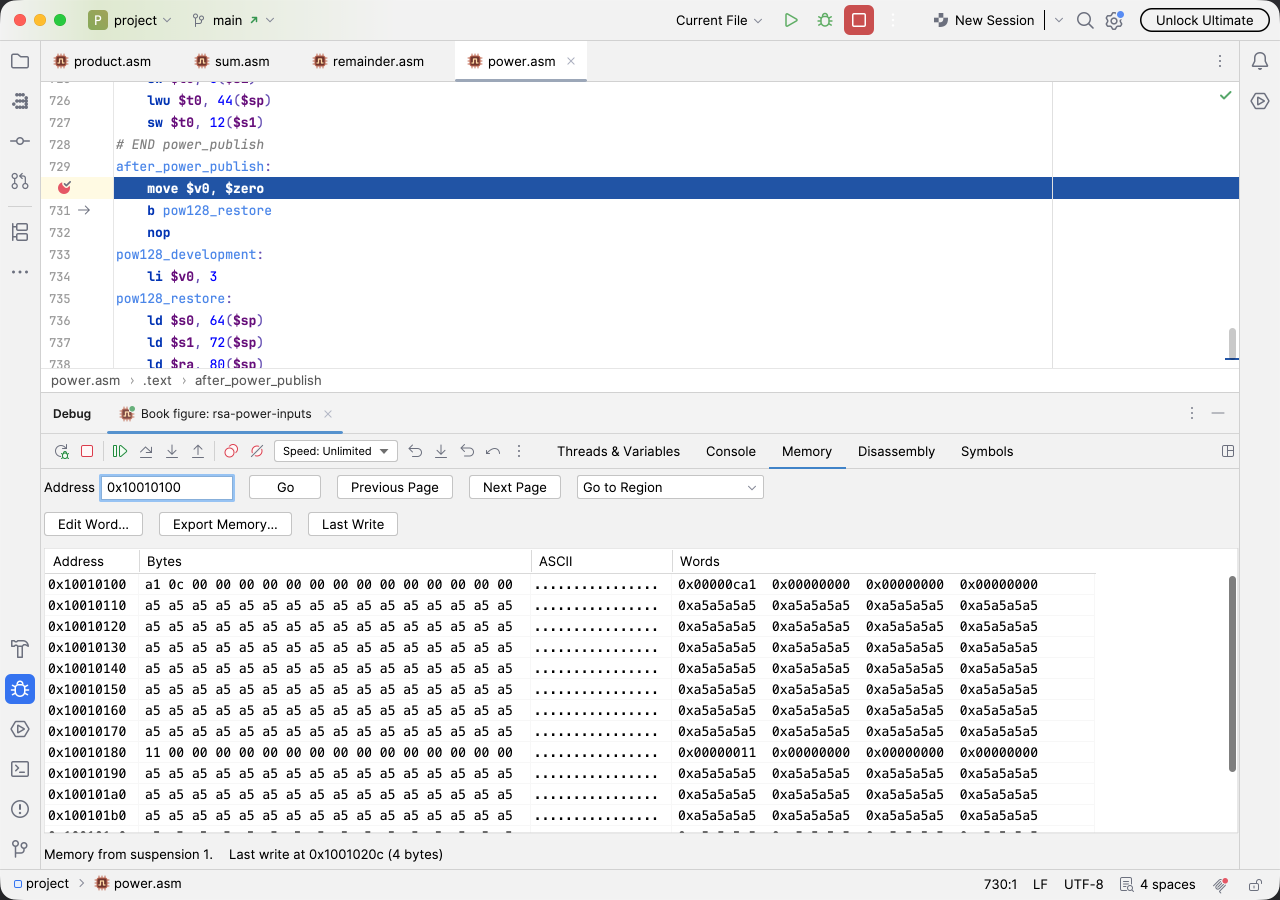
\includegraphics[width=0.84\linewidth,artifact,trim={\MARSrsapowerexponentLeft{} \MARSrsapowerexponentBottom{} \MARSrsapowerexponentRight{} \MARSrsapowerexponentTop{}},clip]{book/captures/027-rsa-arithmetic/f04/inputs.png}};
    \begin{scope}[shift={(exponent.south west)},x={($(exponent.south east)-(exponent.south west)$)},y={($(exponent.north west)-(exponent.south west)$)}]
      \draw[black,line width=0.7pt] (0.194672131,0.078431373) rectangle (0.997950820,0.490196078);
      \node[draw=black,fill=white,circle,inner sep=1.5pt,font=\footnotesize] at ($(0,0.490196078)+(-3mm,0)$) {6};
    \end{scope}
  \end{tikzpicture}
  \par\smallskip
  \begin{minipage}{\linewidth}
    \small
    \begin{enumerate}
      \setlength{\itemsep}{0pt}
            \setlength{\parsep}{0pt}
      \item The stop at \texttt{after\_power\_publish} follows all four output stores. The supplied success and restore sequence has not executed yet.
      \item \texttt{sp = 0x100106a8} is ninety-six bytes below the caller stack top. Nested helper frames have returned, but this outer frame remains allocated.
      \item The complete output is \texttt{e6 0a} followed by fourteen zero bytes: the little-endian four-limb representation of 2790. The upper limbs are part of the result contract, not unspecified padding.
      \item The private exponent begins eight bytes into the first row and spans sixteen zero bytes. The accumulator starts eight bytes into the second row and begins \texttt{e6 0a}. These are private copies; the original exponent remains unchanged.
      \item The original modulus row begins \texttt{a1 0c}, representing 3233. Independently, \mbox{$65^{17}\bmod 3233=2790$}.
      \item The original exponent row begins \texttt{11}, representing 17. Continuing restores saved registers and the stack pointer before returning success; the caller then publishes its status separately.
    \end{enumerate}
  \end{minipage}
  \caption{Modular power publishes its result before restoring the private frame.}
  \label{capture:027-rsa-arithmetic-f04}
  \label{rsa-f04}
\end{figure}
\par
